% Options for packages loaded elsewhere
\PassOptionsToPackage{unicode}{hyperref}
\PassOptionsToPackage{hyphens}{url}
%
\documentclass[
]{article}
\usepackage{lmodern}
\usepackage{amssymb,amsmath}
\usepackage{ifxetex,ifluatex}
\ifnum 0\ifxetex 1\fi\ifluatex 1\fi=0 % if pdftex
  \usepackage[T1]{fontenc}
  \usepackage[utf8]{inputenc}
  \usepackage{textcomp} % provide euro and other symbols
\else % if luatex or xetex
  \usepackage{unicode-math}
  \defaultfontfeatures{Scale=MatchLowercase}
  \defaultfontfeatures[\rmfamily]{Ligatures=TeX,Scale=1}
\fi
% Use upquote if available, for straight quotes in verbatim environments
\IfFileExists{upquote.sty}{\usepackage{upquote}}{}
\IfFileExists{microtype.sty}{% use microtype if available
  \usepackage[]{microtype}
  \UseMicrotypeSet[protrusion]{basicmath} % disable protrusion for tt fonts
}{}
\makeatletter
\@ifundefined{KOMAClassName}{% if non-KOMA class
  \IfFileExists{parskip.sty}{%
    \usepackage{parskip}
  }{% else
    \setlength{\parindent}{0pt}
    \setlength{\parskip}{6pt plus 2pt minus 1pt}}
}{% if KOMA class
  \KOMAoptions{parskip=half}}
\makeatother
\usepackage{xcolor}
\IfFileExists{xurl.sty}{\usepackage{xurl}}{} % add URL line breaks if available
\IfFileExists{bookmark.sty}{\usepackage{bookmark}}{\usepackage{hyperref}}
\hypersetup{
  pdftitle={Homework4\_JKGWAS},
  pdfauthor={Pabitra Joshi and Lindsey Kornowske},
  hidelinks,
  pdfcreator={LaTeX via pandoc}}
\urlstyle{same} % disable monospaced font for URLs
\usepackage[margin=1in]{geometry}
\usepackage{color}
\usepackage{fancyvrb}
\newcommand{\VerbBar}{|}
\newcommand{\VERB}{\Verb[commandchars=\\\{\}]}
\DefineVerbatimEnvironment{Highlighting}{Verbatim}{commandchars=\\\{\}}
% Add ',fontsize=\small' for more characters per line
\usepackage{framed}
\definecolor{shadecolor}{RGB}{248,248,248}
\newenvironment{Shaded}{\begin{snugshade}}{\end{snugshade}}
\newcommand{\AlertTok}[1]{\textcolor[rgb]{0.94,0.16,0.16}{#1}}
\newcommand{\AnnotationTok}[1]{\textcolor[rgb]{0.56,0.35,0.01}{\textbf{\textit{#1}}}}
\newcommand{\AttributeTok}[1]{\textcolor[rgb]{0.77,0.63,0.00}{#1}}
\newcommand{\BaseNTok}[1]{\textcolor[rgb]{0.00,0.00,0.81}{#1}}
\newcommand{\BuiltInTok}[1]{#1}
\newcommand{\CharTok}[1]{\textcolor[rgb]{0.31,0.60,0.02}{#1}}
\newcommand{\CommentTok}[1]{\textcolor[rgb]{0.56,0.35,0.01}{\textit{#1}}}
\newcommand{\CommentVarTok}[1]{\textcolor[rgb]{0.56,0.35,0.01}{\textbf{\textit{#1}}}}
\newcommand{\ConstantTok}[1]{\textcolor[rgb]{0.00,0.00,0.00}{#1}}
\newcommand{\ControlFlowTok}[1]{\textcolor[rgb]{0.13,0.29,0.53}{\textbf{#1}}}
\newcommand{\DataTypeTok}[1]{\textcolor[rgb]{0.13,0.29,0.53}{#1}}
\newcommand{\DecValTok}[1]{\textcolor[rgb]{0.00,0.00,0.81}{#1}}
\newcommand{\DocumentationTok}[1]{\textcolor[rgb]{0.56,0.35,0.01}{\textbf{\textit{#1}}}}
\newcommand{\ErrorTok}[1]{\textcolor[rgb]{0.64,0.00,0.00}{\textbf{#1}}}
\newcommand{\ExtensionTok}[1]{#1}
\newcommand{\FloatTok}[1]{\textcolor[rgb]{0.00,0.00,0.81}{#1}}
\newcommand{\FunctionTok}[1]{\textcolor[rgb]{0.00,0.00,0.00}{#1}}
\newcommand{\ImportTok}[1]{#1}
\newcommand{\InformationTok}[1]{\textcolor[rgb]{0.56,0.35,0.01}{\textbf{\textit{#1}}}}
\newcommand{\KeywordTok}[1]{\textcolor[rgb]{0.13,0.29,0.53}{\textbf{#1}}}
\newcommand{\NormalTok}[1]{#1}
\newcommand{\OperatorTok}[1]{\textcolor[rgb]{0.81,0.36,0.00}{\textbf{#1}}}
\newcommand{\OtherTok}[1]{\textcolor[rgb]{0.56,0.35,0.01}{#1}}
\newcommand{\PreprocessorTok}[1]{\textcolor[rgb]{0.56,0.35,0.01}{\textit{#1}}}
\newcommand{\RegionMarkerTok}[1]{#1}
\newcommand{\SpecialCharTok}[1]{\textcolor[rgb]{0.00,0.00,0.00}{#1}}
\newcommand{\SpecialStringTok}[1]{\textcolor[rgb]{0.31,0.60,0.02}{#1}}
\newcommand{\StringTok}[1]{\textcolor[rgb]{0.31,0.60,0.02}{#1}}
\newcommand{\VariableTok}[1]{\textcolor[rgb]{0.00,0.00,0.00}{#1}}
\newcommand{\VerbatimStringTok}[1]{\textcolor[rgb]{0.31,0.60,0.02}{#1}}
\newcommand{\WarningTok}[1]{\textcolor[rgb]{0.56,0.35,0.01}{\textbf{\textit{#1}}}}
\usepackage{graphicx}
\makeatletter
\def\maxwidth{\ifdim\Gin@nat@width>\linewidth\linewidth\else\Gin@nat@width\fi}
\def\maxheight{\ifdim\Gin@nat@height>\textheight\textheight\else\Gin@nat@height\fi}
\makeatother
% Scale images if necessary, so that they will not overflow the page
% margins by default, and it is still possible to overwrite the defaults
% using explicit options in \includegraphics[width, height, ...]{}
\setkeys{Gin}{width=\maxwidth,height=\maxheight,keepaspectratio}
% Set default figure placement to htbp
\makeatletter
\def\fps@figure{htbp}
\makeatother
\setlength{\emergencystretch}{3em} % prevent overfull lines
\providecommand{\tightlist}{%
  \setlength{\itemsep}{0pt}\setlength{\parskip}{0pt}}
\setcounter{secnumdepth}{-\maxdimen} % remove section numbering

\title{Homework4\_JKGWAS}
\author{Pabitra Joshi and Lindsey Kornowske}
\date{23 March 2021}

\begin{document}
\maketitle

{
\setcounter{tocdepth}{6}
\tableofcontents
}
\begin{figure*}[htbp]
\begin{center}

\includegraphics[width = 0.3\textwidth]{JKGWAS_logo.png}
  \caption{JKGWAS Package Logo}
  \label{fig:logo}
\end{center}
\end{figure*}

\hypertarget{data-and-functions}{%
\section{Data and Functions}\label{data-and-functions}}

The GAPIT demo datasets were used for this assignment. They are
available from ``\url{http://www.zzlab.net/GAPIT/index.html}'' All
credit for these data belong to the Zhiwu Zhang Laboratory.

\begin{Shaded}
\begin{Highlighting}[]
\KeywordTok{library}\NormalTok{(compiler); }\CommentTok{\#need for R version 4.0.4}
\KeywordTok{source}\NormalTok{(}\StringTok{"http://www.zzlab.net/StaGen/2021/R/G2P.R"}\NormalTok{);}
\KeywordTok{source}\NormalTok{(}\StringTok{"http://www.zzlab.net/StaGen/2021/R/GWASbyCor.R"}\NormalTok{);}
\KeywordTok{source}\NormalTok{(}\StringTok{"./../functions/HW4\_JKGWAS\_functions.R"}\NormalTok{);}

\CommentTok{\# Genotype Data}
\NormalTok{X =}\StringTok{ }\KeywordTok{read.csv}\NormalTok{(}\DataTypeTok{file =} \StringTok{"./../datasets/mdp\_numeric.txt"}\NormalTok{, }\DataTypeTok{header =} \OtherTok{TRUE}\NormalTok{, }\DataTypeTok{sep =}\StringTok{""}\NormalTok{);}
\CommentTok{\# Phenotype Data}
\NormalTok{y =}\StringTok{ }\KeywordTok{read.csv}\NormalTok{(}\DataTypeTok{file =} \StringTok{"./../datasets/CROPS545\_Phenotype.txt"}\NormalTok{, }\DataTypeTok{header =} \OtherTok{TRUE}\NormalTok{, }\DataTypeTok{sep =} \StringTok{""}\NormalTok{);}
\CommentTok{\# Covariates Data}
\NormalTok{CV =}\StringTok{ }\KeywordTok{read.csv}\NormalTok{(}\DataTypeTok{file =} \StringTok{"./../datasets/CROPS545\_Covariates.txt"}\NormalTok{, }\DataTypeTok{header =} \OtherTok{TRUE}\NormalTok{, }\DataTypeTok{sep =} \StringTok{""}\NormalTok{);}
\CommentTok{\# SNP information data}
\NormalTok{SNP =}\StringTok{ }\KeywordTok{read.csv}\NormalTok{(}\DataTypeTok{file =} \StringTok{"./../datasets/mdp\_SNP\_information.txt"}\NormalTok{, }\DataTypeTok{header =} \OtherTok{TRUE}\NormalTok{, }\DataTypeTok{sep =} \StringTok{""}\NormalTok{);}
\end{Highlighting}
\end{Shaded}

\hypertarget{question-1-and-2}{%
\section{Question 1 and 2}\label{question-1-and-2}}

\textbf{(1) The package should contain at least three input: y, X , and C that are R objects of numeric data frame. Their dimensions are n by 1, n by m, and n by t corresponding to phenotype, genotype and covariate data, where n is number of individuals, m is number of markers, and t is number of covariates. The function should return probability values with dimension of 1 by m for the association tests between phenotype and markers. Markers are tested one at a time with covariates in C included as covariates (15 points).
(2) The package should perform PCA and incorporate PCs as cofactors for GWAS.  Your package should also automatically exclude the PCs that are in linear dependent to the covariates provided by users. (25 points).}

\begin{Shaded}
\begin{Highlighting}[]
\CommentTok{\#library(devtools)}
\CommentTok{\#install\_github("lindseymaek/HORT545/JKGWAS")}
\KeywordTok{library}\NormalTok{(JKGWAS); }\CommentTok{\#JKGWAS package}
\end{Highlighting}
\end{Shaded}

\hypertarget{jkgwas-summary}{%
\subsection{JKGWAS Summary}\label{jkgwas-summary}}

The JKGWAS Package contains four functions that are summarized briefly
as follows, more information is located in the JKGWAS Package
documentation:

\par

\textbullet{JKPCA takes genotype (X) data and covariate data (CV), computes the PCA on X, then automatically removes PCs that are linearly dependent to the CVs by method of comparing matrix rank. PCs are removed from the matrix in succesion and those that do not change the rank by removal are determined to be linearly independent because they do not provide additional information.}

\par

\textbullet{JKGLM takes phenotype (y), genotype (X), covariate (CV), and principal component (PC) inputs (ideally provided from JKPCA) and returns p-values calculated for the association tests between the phenotype and SNPs}

\par
\textbullet{JKQQ takes the pvalues from JKGLM and visualizes them by QQ plot. Expected p-values of length m are simulated from the continuous distribution.}\par
\textbullet{JKManhattan visualizes the pvalues from JKGLM by Manhattan plot. User input QTNs can also be visualized. The significance threshold can be set, or it will default to Bonferoni correction for alpha = 0.05}\par

\hypertarget{question-3}{%
\section{Question 3}\label{question-3}}

\textbf{(3) Develop a user manual and tutorials. Name your package and create a logo. (20 points).}

The JKGWAS package is named for Pabitra Joshi and Lindsey Kornowske, the
label is displayed in Figure \ref{fig:logo}.

The JKGWAS package documentation is provided in a separate file,
``JKGWAS\_0.1.0\_PackageDocumentation.pdf'' and further information
about its use are provided in the user tutorial,
``JKGWAS\_UserTutorial.pdf''

\hypertarget{question-4}{%
\section{Question 4}\label{question-4}}

\textbf{(4) Perform GWAS on the data provided or your own data which must contain cofactors (15 points).}

First, GWAS was performed with the phenotype data provided. In the
Manhattan plot below, we can see that 4 SNP were detected, but because
we do not have information about the QTNs, we do not know whether these
significant observations represent true positives or not. Next, we use a
simulated phenotype to better assess the performance of the JKGWAS
approach.

\hypertarget{gwas-with-provided-phenotype-data}{%
\subsection{GWAS with provided phenotype
data}\label{gwas-with-provided-phenotype-data}}

\begin{Shaded}
\begin{Highlighting}[]
\CommentTok{\#\# Get Principal Components with JKPCA()}
\NormalTok{PC =}\StringTok{ }\KeywordTok{JKPCA}\NormalTok{(X, CV, }\DataTypeTok{npc =} \DecValTok{10}\NormalTok{);}

\CommentTok{\#\# Perform GWAS by GLM with JKGLM()}
\NormalTok{Pvals =}\StringTok{ }\KeywordTok{JKGLM}\NormalTok{(}\DataTypeTok{X =}\NormalTok{ X, }\DataTypeTok{y =}\NormalTok{ y, CV, PC);}
\end{Highlighting}
\end{Shaded}

\hypertarget{qq-plot}{%
\subsubsection{QQ Plot}\label{qq-plot}}

\begin{Shaded}
\begin{Highlighting}[]
\CommentTok{\#\# Visualize GWAS by QQ Plot with JKQQ()}
\KeywordTok{JKQQ}\NormalTok{(Pvals);}
\end{Highlighting}
\end{Shaded}

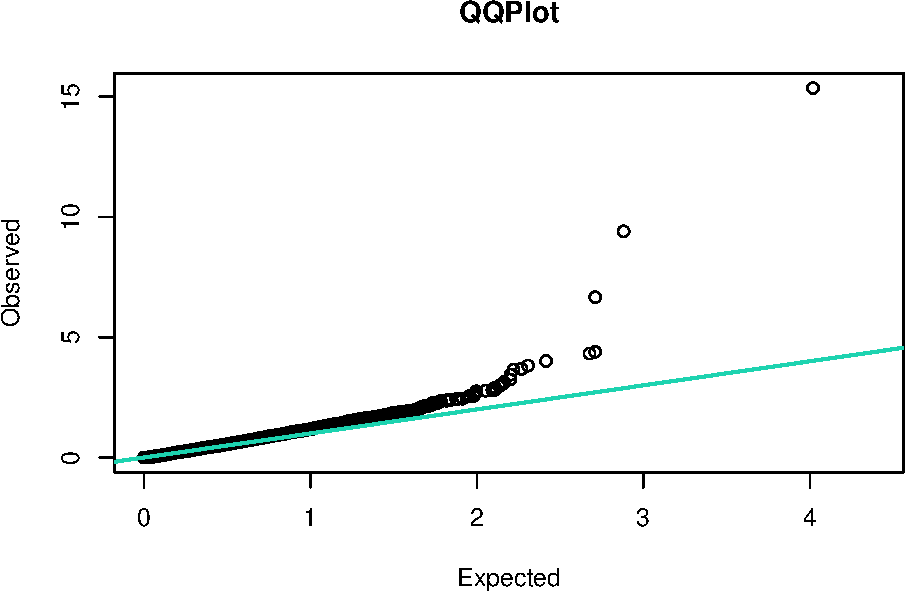
\includegraphics{Homework4_JKGWAS_files/figure-latex/unnamed-chunk-4-1.pdf}

\hypertarget{genome-wide-threshold}{%
\subsubsection{Genome-wide Threshold}\label{genome-wide-threshold}}

With the Bonferroni correction, our threshold is as follows:

\begin{Shaded}
\begin{Highlighting}[]
\NormalTok{sig.threshold =}\StringTok{ }\FloatTok{0.05}\OperatorTok{/}\KeywordTok{length}\NormalTok{(Pvals);}
\NormalTok{sig.threshold;}
\end{Highlighting}
\end{Shaded}

\begin{verbatim}
## [1] 1.616554e-05
\end{verbatim}

\hypertarget{list-of-associated-snp}{%
\subsubsection{List of Associated SNP}\label{list-of-associated-snp}}

Because the genomic data and SNP data are in the same order, we can
index the significant p-values in the SNP data.

\begin{Shaded}
\begin{Highlighting}[]
\NormalTok{SNP[Pvals}\OperatorTok{\textless{}}\NormalTok{sig.threshold,];}
\end{Highlighting}
\end{Shaded}

\begin{verbatim}
##              SNP Chromosome Position
## 937   PZA00615.3          3  1882847
## 1013  PZA02699.1          3 63847564
## 2715 PZA03058.17          9 19292988
## 2717 PZA03058.21          9 19293212
\end{verbatim}

\hypertarget{maf-of-associated-snp}{%
\subsubsection{MAF of Associated SNP}\label{maf-of-associated-snp}}

\begin{Shaded}
\begin{Highlighting}[]
\NormalTok{X.num =}\StringTok{ }\NormalTok{dplyr}\OperatorTok{::}\KeywordTok{select\_if}\NormalTok{(X, is.numeric); }

\CommentTok{\#save associated SNP genomic data to dataframe}
\NormalTok{SNP.GD =}\StringTok{ }\NormalTok{X.num[,Pvals}\OperatorTok{\textless{}}\NormalTok{sig.threshold];}

\CommentTok{\#calculate MAF and store in array}
\NormalTok{MAF =}\StringTok{ }\KeywordTok{apply}\NormalTok{(SNP.GD, }\DecValTok{2}\NormalTok{, }\ControlFlowTok{function}\NormalTok{(x)}
\NormalTok{  \{}
\NormalTok{  allele.freq1 =}\StringTok{ }\NormalTok{(}\KeywordTok{sum}\NormalTok{(x}\OperatorTok{==}\DecValTok{0}\NormalTok{)}\OperatorTok{*}\DecValTok{2} \OperatorTok{+}\StringTok{ }\KeywordTok{sum}\NormalTok{(x}\OperatorTok{==}\DecValTok{1}\NormalTok{))}\OperatorTok{/}\NormalTok{(}\KeywordTok{sum}\NormalTok{(}\OperatorTok{!}\KeywordTok{is.na}\NormalTok{(x))}\OperatorTok{*}\DecValTok{2}\NormalTok{);}
\NormalTok{  allele.freq2 =}\StringTok{ }\NormalTok{(}\KeywordTok{sum}\NormalTok{(x}\OperatorTok{==}\DecValTok{2}\NormalTok{)}\OperatorTok{*}\DecValTok{2} \OperatorTok{+}\StringTok{ }\KeywordTok{sum}\NormalTok{(x}\OperatorTok{==}\DecValTok{1}\NormalTok{))}\OperatorTok{/}\NormalTok{(}\KeywordTok{sum}\NormalTok{(}\OperatorTok{!}\KeywordTok{is.na}\NormalTok{(x))}\OperatorTok{*}\DecValTok{2}\NormalTok{);}
  
  \KeywordTok{return}\NormalTok{(}\KeywordTok{min}\NormalTok{(allele.freq1, allele.freq2));}
\NormalTok{  \})}

\NormalTok{MAF;}
\end{Highlighting}
\end{Shaded}

\begin{verbatim}
##  PZA00615.3  PZA02699.1 PZA03058.17 PZA03058.21 
##   0.1103203   0.3451957   0.1120996   0.1032028
\end{verbatim}

The MAFs for the significant QTNs are shown above. In this case, the MAF
is fairly low for 3/4 associated SNP, which tells us that these variants
are comparably rare to the major alleles.

\hypertarget{manhattan-plot}{%
\subsubsection{Manhattan Plot}\label{manhattan-plot}}

\begin{Shaded}
\begin{Highlighting}[]
\CommentTok{\#\# Visualize GWAS by Manhattan Plot with JKManhattan()}
\KeywordTok{JKManhattan}\NormalTok{(}\DataTypeTok{Pvals =}\NormalTok{ Pvals, }\DataTypeTok{SNP =}\NormalTok{ SNP,}\DataTypeTok{sigcutoff =} \OtherTok{NULL}\NormalTok{ );}
\end{Highlighting}
\end{Shaded}

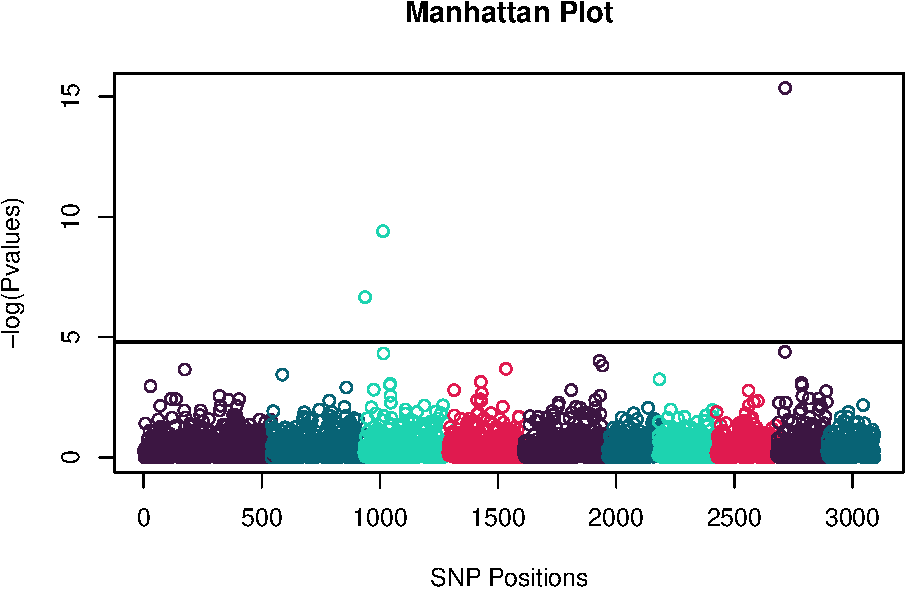
\includegraphics{Homework4_JKGWAS_files/figure-latex/unnamed-chunk-8-1.pdf}

\hypertarget{gwas-with-simulated-phenotype}{%
\subsection{GWAS with simulated
phenotype}\label{gwas-with-simulated-phenotype}}

\begin{Shaded}
\begin{Highlighting}[]
\KeywordTok{set.seed}\NormalTok{(}\DecValTok{12}\NormalTok{);}
\CommentTok{\#simulate phenotype with heritability value 0.75}
\NormalTok{G2P.sim =}\StringTok{ }\KeywordTok{G2P}\NormalTok{(}\DataTypeTok{X=}\NormalTok{ X.num,}
             \DataTypeTok{h2=} \FloatTok{0.75}\NormalTok{,}
             \DataTypeTok{alpha=}\DecValTok{1}\NormalTok{,}
             \DataTypeTok{NQTN=}\DecValTok{10}\NormalTok{,}
             \DataTypeTok{distribution=}\StringTok{"norm"}\NormalTok{);}

\CommentTok{\#save the phenotype to variable for the JKGLM() function}
\NormalTok{G2P.y =}\StringTok{ }\KeywordTok{as.data.frame}\NormalTok{(G2P.sim}\OperatorTok{$}\NormalTok{y);}

\NormalTok{G2P.qtn =}\StringTok{ }\NormalTok{G2P.sim}\OperatorTok{$}\NormalTok{QTN.position; }

\CommentTok{\#perform GWAS by GLM with JKGLM}
\NormalTok{Pvals.sim =}\StringTok{ }\KeywordTok{JKGLM}\NormalTok{(}\DataTypeTok{X =}\NormalTok{ X, }\DataTypeTok{y =}\NormalTok{ G2P.y, CV, PC);}
\end{Highlighting}
\end{Shaded}

\hypertarget{qq-plot-1}{%
\subsubsection{QQ Plot}\label{qq-plot-1}}

\begin{Shaded}
\begin{Highlighting}[]
\CommentTok{\#\# Visualize GWAS by QQ Plot with JKQQ()}
\KeywordTok{JKQQ}\NormalTok{(Pvals.sim);}
\end{Highlighting}
\end{Shaded}

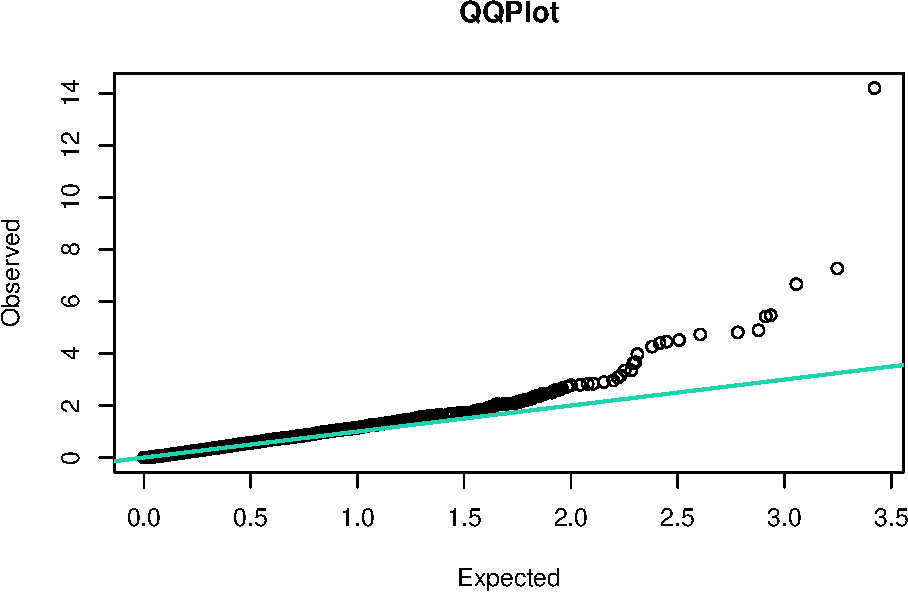
\includegraphics{Homework4_JKGWAS_files/figure-latex/unnamed-chunk-10-1.pdf}
Unlike the provided data, the simulated data shows a more dramatic
departure from the expected values. We can anticipate more associated
SNPs but also more false positives.

\hypertarget{list-of-associated-snp-1}{%
\subsubsection{List of Associated SNP}\label{list-of-associated-snp-1}}

\begin{Shaded}
\begin{Highlighting}[]
\NormalTok{SNP[Pvals.sim}\OperatorTok{\textless{}}\NormalTok{sig.threshold,];}
\end{Highlighting}
\end{Shaded}

\begin{verbatim}
##              SNP Chromosome  Position
## 336   PZB00011.1          1 233401031
## 339   PZB00116.2          1 233401241
## 450   PZA03188.2          1 280719532
## 1093  PZB01683.2          3 156252241
## 1160 PZA00482.10          3 180294773
## 2907  PZB01301.7         10   9748233
## 2909  PZB01301.5         10   9748559
\end{verbatim}

\hypertarget{maf-of-associated-snp-1}{%
\subsubsection{MAF of Associated SNP}\label{maf-of-associated-snp-1}}

\begin{Shaded}
\begin{Highlighting}[]
\CommentTok{\#save associated SNP genomic data to dataframe}
\NormalTok{SNP.GD =}\StringTok{ }\NormalTok{X.num[,Pvals.sim}\OperatorTok{\textless{}}\NormalTok{sig.threshold];}

\CommentTok{\#calculate MAF and store in array}
\NormalTok{MAF =}\StringTok{ }\KeywordTok{apply}\NormalTok{(SNP.GD, }\DecValTok{2}\NormalTok{, }\ControlFlowTok{function}\NormalTok{(x)}
\NormalTok{  \{}
\NormalTok{  allele.freq1 =}\StringTok{ }\NormalTok{(}\KeywordTok{sum}\NormalTok{(x}\OperatorTok{==}\DecValTok{0}\NormalTok{)}\OperatorTok{*}\DecValTok{2} \OperatorTok{+}\StringTok{ }\KeywordTok{sum}\NormalTok{(x}\OperatorTok{==}\DecValTok{1}\NormalTok{))}\OperatorTok{/}\NormalTok{(}\KeywordTok{sum}\NormalTok{(}\OperatorTok{!}\KeywordTok{is.na}\NormalTok{(x))}\OperatorTok{*}\DecValTok{2}\NormalTok{);}
\NormalTok{  allele.freq2 =}\StringTok{ }\NormalTok{(}\KeywordTok{sum}\NormalTok{(x}\OperatorTok{==}\DecValTok{2}\NormalTok{)}\OperatorTok{*}\DecValTok{2} \OperatorTok{+}\StringTok{ }\KeywordTok{sum}\NormalTok{(x}\OperatorTok{==}\DecValTok{1}\NormalTok{))}\OperatorTok{/}\NormalTok{(}\KeywordTok{sum}\NormalTok{(}\OperatorTok{!}\KeywordTok{is.na}\NormalTok{(x))}\OperatorTok{*}\DecValTok{2}\NormalTok{);}
  
  \KeywordTok{return}\NormalTok{(}\KeywordTok{min}\NormalTok{(allele.freq1, allele.freq2));}
\NormalTok{  \})}

\NormalTok{MAF;}
\end{Highlighting}
\end{Shaded}

\begin{verbatim}
##  PZB00011.1  PZB00116.2  PZA03188.2  PZB01683.2 PZA00482.10  PZB01301.7 
##   0.4448399   0.4430605   0.4056940   0.1494662   0.4412811   0.3647687 
##  PZB01301.5 
##   0.3523132
\end{verbatim}

In the case of the simulated data, the MAF is much closer to 0.5, for at
least half of the associated SNPs. These alleles do not represent rare
variants as compared with the provided phenotype data.

\hypertarget{manhattan-plot-1}{%
\subsubsection{Manhattan Plot}\label{manhattan-plot-1}}

\begin{Shaded}
\begin{Highlighting}[]
\CommentTok{\#\# Visualize GWAS by Manhattan Plot with JKManhattan()}
\KeywordTok{JKManhattan}\NormalTok{(}\DataTypeTok{Pvals =}\NormalTok{ Pvals.sim, }\DataTypeTok{SNP =}\NormalTok{ SNP, }\DataTypeTok{sigcutoff =} \OtherTok{NULL}\NormalTok{, }\DataTypeTok{QTN =}\NormalTok{ G2P.qtn);}
\end{Highlighting}
\end{Shaded}

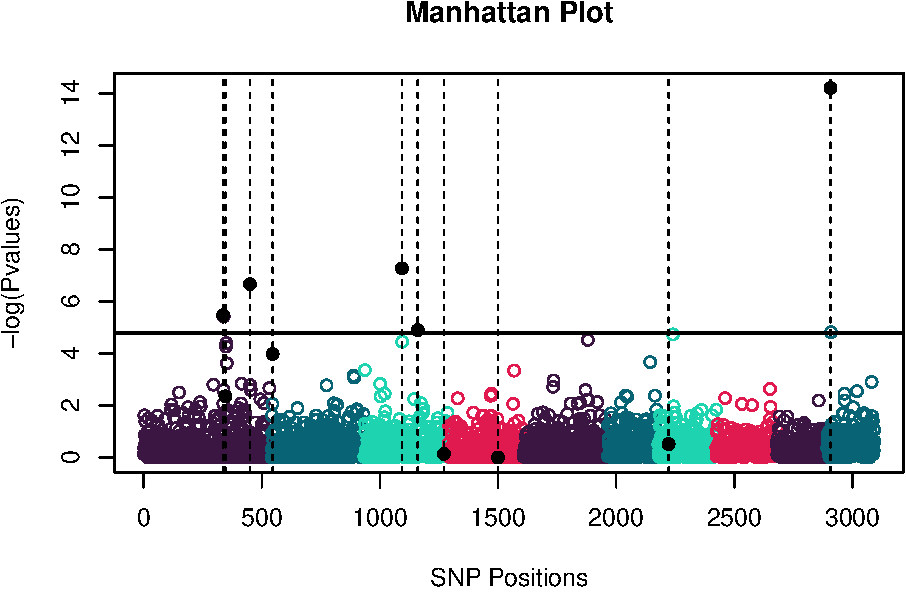
\includegraphics{Homework4_JKGWAS_files/figure-latex/unnamed-chunk-13-1.pdf}

If we use a simulated phenotype instead of the provided phenotype data,
50\% of our 10 QTN are detected correctly. meaning that there is a 50\%
false negative rate. With 5 QTN detected out of 7 associated SNPs total,
that is a True Positive rate of 71.4\%.

\hypertarget{question-5}{%
\section{Question 5}\label{question-5}}

\textbf{(5) Demonstrate that your method is superior to the competing method (GWASbyCor) through simulation with at least 30 replicates (25 points).}

See file HW4\_JKGWAS\_functions.R for the function source code.

In order to compare GWASbyCor and GWASbyGLM, we created a function
called compareGWASnTimes. The function arguments are:

\par

\textbullet{n, the number of times to run the simulation}

\par

\textbullet{X, the numeric genomic data}

\par

\textbullet{qtn, the number of qtns to be simulated}

\par
\textbullet{CV, the covariate matrix to be passed to the JKGLM function. The default value is NULL }\par
\textbullet{PC, the principal component matrix to be passed to the JKGLM function. The default value is NULL }\par

For each iteration, the G2P function simulates the phenotype for X with
a heritability of 0.75. Then, the output phenotype is used to compute
the GWAS by cor and the GWAS by GLM. The number of True Positives, as
well as the True Positive Rate, which is calculated as the number of
QTNs that is correctly identified out of all significant SNPs (p-value
is smaller than 0.05/total pvalues, Bonferroni correction is automatic).
These two dataframes are output as a list, where the first item is the
count of true positive QTNs and the second item is the true positive
rate.

\begin{Shaded}
\begin{Highlighting}[]
\CommentTok{\# Run the simulation comparison 30 times}
\KeywordTok{set.seed}\NormalTok{(}\DecValTok{8345}\NormalTok{);}
\NormalTok{test =}\StringTok{ }\KeywordTok{compareGWASnTimes}\NormalTok{(}\DataTypeTok{n=}\DecValTok{30}\NormalTok{, }\DataTypeTok{X =}\NormalTok{ X, }\DataTypeTok{qtn =} \DecValTok{10}\NormalTok{, }\DataTypeTok{CV =}\NormalTok{ CV, }\DataTypeTok{PC =}\NormalTok{ PC);}
\CommentTok{\#test;}
\end{Highlighting}
\end{Shaded}

The output of the function compareGWASnTimes() is a list containing
lists for the results for GWAS by COR and GWAS by GLM for 4 items; 1)
the number of QTNs detected among the significant SNPs 2) the true
positive rate 3) the number of non-QTN SNPs detectected among the
significant SNPs and 4) the false positive rate.

\hypertarget{true-positive-rate}{%
\subsection{True Positive Rate}\label{true-positive-rate}}

\begin{Shaded}
\begin{Highlighting}[]
\KeywordTok{mean}\NormalTok{(test[[}\DecValTok{2}\NormalTok{]]}\OperatorTok{$}\NormalTok{COR); }\CommentTok{\#mean TPR for Cor is 0.44}
\end{Highlighting}
\end{Shaded}

\begin{verbatim}
## [1] 0.4387465
\end{verbatim}

\begin{Shaded}
\begin{Highlighting}[]
\KeywordTok{mean}\NormalTok{(test[[}\DecValTok{2}\NormalTok{]]}\OperatorTok{$}\NormalTok{GLM); }\CommentTok{\#mean TPR for GLM is 0.71}
\end{Highlighting}
\end{Shaded}

\begin{verbatim}
## [1] 0.7089453
\end{verbatim}

\begin{Shaded}
\begin{Highlighting}[]
\KeywordTok{mean}\NormalTok{(test[[}\DecValTok{4}\NormalTok{]]}\OperatorTok{$}\NormalTok{COR); }\CommentTok{\#mean FPR for Cor is 0.56}
\end{Highlighting}
\end{Shaded}

\begin{verbatim}
## [1] 0.5592927
\end{verbatim}

\begin{Shaded}
\begin{Highlighting}[]
\KeywordTok{mean}\NormalTok{(test[[}\DecValTok{4}\NormalTok{]]}\OperatorTok{$}\NormalTok{GLM); }\CommentTok{\#mean FPR for GLM is 0.29}
\end{Highlighting}
\end{Shaded}

\begin{verbatim}
## [1] 0.2910547
\end{verbatim}

By these calculations, we can see that the standard deviation of the
true positive rate for each method is comparable. The True Positive Rate
is marginally higher for the GWAS by GLM than the GWAS by Cor.

\hypertarget{statistical-inference}{%
\subsection{Statistical Inference}\label{statistical-inference}}

H\(_{o}\); the mean rates are equal

\par

H\(_{1}\); the mean rates are not equal

significance threshold: 0.05

\hypertarget{true-positive-rate-1}{%
\subsubsection{True positive rate}\label{true-positive-rate-1}}

p = 1.777e-05

Reject the null hypothesis; there is sufficient evidence to suggest that
the mean true positive rates for GWAS by Cor and GWAS by JKGWAS are
different. The mean TPR for JKGWAS was 0.71, almost double that for GWAS
by Cor (0.44).

\begin{Shaded}
\begin{Highlighting}[]
\KeywordTok{t.test}\NormalTok{(}\DataTypeTok{x =}\NormalTok{ test[[}\DecValTok{2}\NormalTok{]]}\OperatorTok{$}\NormalTok{COR, }\DataTypeTok{y =}\NormalTok{ test[[}\DecValTok{2}\NormalTok{]]}\OperatorTok{$}\NormalTok{GLM)}
\end{Highlighting}
\end{Shaded}

\begin{verbatim}
## 
##  Welch Two Sample t-test
## 
## data:  test[[2]]$COR and test[[2]]$GLM
## t = -4.6905, df = 56.355, p-value = 1.777e-05
## alternative hypothesis: true difference in means is not equal to 0
## 95 percent confidence interval:
##  -0.3855803 -0.1548172
## sample estimates:
## mean of x mean of y 
## 0.4387465 0.7089453
\end{verbatim}

\hypertarget{false-positive-rate}{%
\subsubsection{False positive rate}\label{false-positive-rate}}

p-value = 1.883e-05

Reject the null hypothesis; there is sufficient evidence to suggest that
the mean false positive rates for GWAS by Cor and GWAS by JKGWAS are
different. The mean FPR for JKGWAS was 0.29, almost half that for GWAS
by Cor (0.56).

\begin{Shaded}
\begin{Highlighting}[]
\KeywordTok{t.test}\NormalTok{(}\DataTypeTok{x =}\NormalTok{ test[[}\DecValTok{4}\NormalTok{]]}\OperatorTok{$}\NormalTok{COR, }\DataTypeTok{y =}\NormalTok{ test[[}\DecValTok{4}\NormalTok{]]}\OperatorTok{$}\NormalTok{GLM);}
\end{Highlighting}
\end{Shaded}

\begin{verbatim}
## 
##  Welch Two Sample t-test
## 
## data:  test[[4]]$COR and test[[4]]$GLM
## t = 4.6732, df = 56.465, p-value = 1.883e-05
## alternative hypothesis: true difference in means is not equal to 0
## 95 percent confidence interval:
##  0.1532735 0.3832024
## sample estimates:
## mean of x mean of y 
## 0.5592927 0.2910547
\end{verbatim}

\hypertarget{extra-credit}{%
\section{Extra Credit}\label{extra-credit}}

\textbf{(6) Demonstrate that your package is better than BLINK C version (http://zzlab.net/blink) on either statistical power or speed (25 points). }

See file HW4\_JKGWAS\_functions.R for the function source code.

We created two functions to test this data. simBLINKnTimes(), where the
user can input the number of desired iterations, the genomic data, and
the genetic map data, then get the true and false positive rates, as
well as the times required for the GWAS by BLINK. simJKGWASnTimes() does
the same thing, but for our JKGWAS function.

Three sets of GAPIT demo datasets from ZZlab were used. In each trial,
both of the functions mentioned above were run 30 times. Then the run
time, true positive rate, and false positive rate were compared by
two-sided t-test for each method to evaluate the null hypothesis of
equal means. Across all three datasets, the computing time varied within
each method, but in each case, the time to complete JKGWAS was
significantly faster than BLINK (alpha = 0.05). The average computing
times for the datasets are reported in the chunks below.

BLINK, however, appears to be worth the additional time cost, because it
was found to have higher power, with a significantly higher True
Positive Rate and a significantly lower False Negative Rate than JKGWAS
in all trials. The average false and true positive rates are reported in
the chunks below.

\begin{Shaded}
\begin{Highlighting}[]
\CommentTok{\#\# Loading BLINK packages and source code}
\KeywordTok{source}\NormalTok{(}\StringTok{"http://zzlab.net/GAPIT/gapit\_functions.txt"}\NormalTok{);}
\KeywordTok{source}\NormalTok{(}\StringTok{"http://zzlab.net/GAPIT/GAPIT.library.R"}\NormalTok{)}
\end{Highlighting}
\end{Shaded}

\hypertarget{dataset-1}{%
\subsection{Dataset 1}\label{dataset-1}}

\begin{Shaded}
\begin{Highlighting}[]
\CommentTok{\#test1 {-} Dataset 1 is the same as is used throughout assignment}
\KeywordTok{set.seed}\NormalTok{(}\DecValTok{1}\NormalTok{);}
\NormalTok{BLINK1 =}\StringTok{ }\KeywordTok{simBLINKnTimes}\NormalTok{(}\DecValTok{30}\NormalTok{, }\DataTypeTok{X =}\NormalTok{ X, }\DataTypeTok{SNP =}\NormalTok{ SNP);}
\KeywordTok{set.seed}\NormalTok{(}\DecValTok{1}\NormalTok{);}
\NormalTok{GLM1 =}\StringTok{ }\KeywordTok{simJKGWASnTimes}\NormalTok{(}\DecValTok{30}\NormalTok{, }\DataTypeTok{X =}\NormalTok{ X, }\DataTypeTok{SNP =}\NormalTok{ SNP);}
\end{Highlighting}
\end{Shaded}

\hypertarget{statistical-inference-1}{%
\subsubsection{Statistical Inference}\label{statistical-inference-1}}

\begin{Shaded}
\begin{Highlighting}[]
\CommentTok{\#compare time}
\KeywordTok{t.test}\NormalTok{(BLINK1}\OperatorTok{$}\NormalTok{BLINK\_Time, GLM1}\OperatorTok{$}\NormalTok{GLM\_Time); }\CommentTok{\# pval \textless{}0.05 JKGLM is faster}
\end{Highlighting}
\end{Shaded}

\begin{verbatim}
## 
##  Welch Two Sample t-test
## 
## data:  BLINK1$BLINK_Time and GLM1$GLM_Time
## t = 14.423, df = 57.187, p-value < 2.2e-16
## alternative hypothesis: true difference in means is not equal to 0
## 95 percent confidence interval:
##  4.107527 5.431890
## sample estimates:
## mean of x mean of y 
## -11.26499 -16.03470
\end{verbatim}

\begin{Shaded}
\begin{Highlighting}[]
\CommentTok{\#compare TPR}
\KeywordTok{t.test}\NormalTok{(BLINK1}\OperatorTok{$}\NormalTok{TPR, GLM1}\OperatorTok{$}\NormalTok{TPR); }\CommentTok{\# pval \textless{}0.05, Blink is higher}
\end{Highlighting}
\end{Shaded}

\begin{verbatim}
## 
##  Welch Two Sample t-test
## 
## data:  BLINK1$TPR and GLM1$TPR
## t = 4.9314, df = 45.33, p-value = 1.139e-05
## alternative hypothesis: true difference in means is not equal to 0
## 95 percent confidence interval:
##  0.1649980 0.3927533
## sample estimates:
## mean of x mean of y 
## 0.8833333 0.6044577
\end{verbatim}

\begin{Shaded}
\begin{Highlighting}[]
\CommentTok{\#compare FPR}
\KeywordTok{t.test}\NormalTok{(BLINK1}\OperatorTok{$}\NormalTok{FPR, GLM1}\OperatorTok{$}\NormalTok{FPR); }\CommentTok{\#pval \textless{}0.05, Blink is lower}
\end{Highlighting}
\end{Shaded}

\begin{verbatim}
## 
##  Welch Two Sample t-test
## 
## data:  BLINK1$FPR and GLM1$FPR
## t = -3.3676, df = 52.682, p-value = 0.001423
## alternative hypothesis: true difference in means is not equal to 0
## 95 percent confidence interval:
##  -0.25256633 -0.06399452
## sample estimates:
## mean of x mean of y 
## 0.1166667 0.2749471
\end{verbatim}

\hypertarget{dataset-2}{%
\subsection{Dataset 2}\label{dataset-2}}

\begin{Shaded}
\begin{Highlighting}[]
\CommentTok{\#test 2 {-} Dataset 2 is from zzlab {-} all files with "2"}
\CommentTok{\# Genotype Data}
\NormalTok{X2 =}\StringTok{ }\KeywordTok{read.csv}\NormalTok{(}\DataTypeTok{file =} \StringTok{"./../datasets/mdp\_numeric2.txt"}\NormalTok{, }\DataTypeTok{header =} \OtherTok{TRUE}\NormalTok{, }\DataTypeTok{sep =}\StringTok{""}\NormalTok{);}
\CommentTok{\# SNP information data}
\NormalTok{SNP2 =}\StringTok{ }\KeywordTok{read.csv}\NormalTok{(}\DataTypeTok{file =} \StringTok{"./../datasets/mdp\_SNP\_information2.txt"}\NormalTok{, }\DataTypeTok{header =} \OtherTok{TRUE}\NormalTok{, }\DataTypeTok{sep =} \StringTok{""}\NormalTok{);}
\end{Highlighting}
\end{Shaded}

\begin{Shaded}
\begin{Highlighting}[]
\KeywordTok{set.seed}\NormalTok{(}\DecValTok{2}\NormalTok{);}
\NormalTok{BLINK2 =}\StringTok{ }\KeywordTok{simBLINKnTimes}\NormalTok{(}\DecValTok{30}\NormalTok{, }\DataTypeTok{X =}\NormalTok{ X2, }\DataTypeTok{SNP =}\NormalTok{ SNP2);}
\KeywordTok{set.seed}\NormalTok{(}\DecValTok{2}\NormalTok{);}
\NormalTok{GLM2 =}\StringTok{ }\KeywordTok{simJKGWASnTimes}\NormalTok{(}\DecValTok{30}\NormalTok{, }\DataTypeTok{X =}\NormalTok{ X2, }\DataTypeTok{SNP =}\NormalTok{ SNP2);}
\end{Highlighting}
\end{Shaded}

\hypertarget{statistical-inference-2}{%
\subsubsection{Statistical Inference}\label{statistical-inference-2}}

\begin{Shaded}
\begin{Highlighting}[]
\CommentTok{\#compare time}
\KeywordTok{t.test}\NormalTok{(BLINK2}\OperatorTok{$}\NormalTok{BLINK\_Time, GLM2}\OperatorTok{$}\NormalTok{GLM\_Time); }\CommentTok{\# pval \textless{}0.05 JKGLM is faster}
\end{Highlighting}
\end{Shaded}

\begin{verbatim}
## 
##  Welch Two Sample t-test
## 
## data:  BLINK2$BLINK_Time and GLM2$GLM_Time
## t = -21.247, df = 30.377, p-value < 2.2e-16
## alternative hypothesis: true difference in means is not equal to 0
## 95 percent confidence interval:
##  -4.212143 -3.473741
## sample estimates:
## mean of x mean of y 
## -8.384335 -4.541393
\end{verbatim}

\begin{Shaded}
\begin{Highlighting}[]
\CommentTok{\#compare TPR}
\KeywordTok{t.test}\NormalTok{(BLINK2}\OperatorTok{$}\NormalTok{TPR, GLM2}\OperatorTok{$}\NormalTok{TPR);}\CommentTok{\# pval \textless{}0.05, Blink is higher}
\end{Highlighting}
\end{Shaded}

\begin{verbatim}
## 
##  Welch Two Sample t-test
## 
## data:  BLINK2$TPR and GLM2$TPR
## t = 6.6553, df = 44.485, p-value = 3.489e-08
## alternative hypothesis: true difference in means is not equal to 0
## 95 percent confidence interval:
##  0.2042788 0.3816603
## sample estimates:
## mean of x mean of y 
## 0.8966402 0.6036706
\end{verbatim}

\begin{Shaded}
\begin{Highlighting}[]
\CommentTok{\#compare FPR}
\KeywordTok{t.test}\NormalTok{(BLINK2}\OperatorTok{$}\NormalTok{FPR, GLM2}\OperatorTok{$}\NormalTok{FPR); }\CommentTok{\#pval \textless{}0.05, Blink is lower}
\end{Highlighting}
\end{Shaded}

\begin{verbatim}
## 
##  Welch Two Sample t-test
## 
## data:  BLINK2$FPR and GLM2$FPR
## t = -5.1322, df = 48.475, p-value = 5.023e-06
## alternative hypothesis: true difference in means is not equal to 0
## 95 percent confidence interval:
##  -0.2823008 -0.1234002
## sample estimates:
## mean of x mean of y 
## 0.1033598 0.3062103
\end{verbatim}

\hypertarget{dataset-3}{%
\subsection{Dataset 3}\label{dataset-3}}

\begin{Shaded}
\begin{Highlighting}[]
\CommentTok{\#test 3 {-} Dataset 3 is from zzlab {-} all files with "3"}
\CommentTok{\# Genotype Data}
\NormalTok{X3 =}\StringTok{ }\KeywordTok{read.csv}\NormalTok{(}\DataTypeTok{file =} \StringTok{"./../datasets/mdp\_numeric3.txt"}\NormalTok{, }\DataTypeTok{header =} \OtherTok{TRUE}\NormalTok{, }\DataTypeTok{sep =}\StringTok{""}\NormalTok{);}
\CommentTok{\# SNP information data}
\NormalTok{SNP3 =}\StringTok{ }\KeywordTok{read.csv}\NormalTok{(}\DataTypeTok{file =} \StringTok{"./../datasets/mdp\_SNP\_information3.txt"}\NormalTok{, }\DataTypeTok{header =} \OtherTok{TRUE}\NormalTok{, }\DataTypeTok{sep =} \StringTok{""}\NormalTok{);}
\end{Highlighting}
\end{Shaded}

\begin{Shaded}
\begin{Highlighting}[]
\KeywordTok{set.seed}\NormalTok{(}\DecValTok{3}\NormalTok{);}
\NormalTok{BLINK3 =}\StringTok{ }\KeywordTok{simBLINKnTimes}\NormalTok{(}\DecValTok{30}\NormalTok{, }\DataTypeTok{X =}\NormalTok{ X3, }\DataTypeTok{SNP =}\NormalTok{ SNP3);}
\KeywordTok{set.seed}\NormalTok{(}\DecValTok{3}\NormalTok{);}
\NormalTok{GLM3 =}\StringTok{ }\KeywordTok{simJKGWASnTimes}\NormalTok{(}\DecValTok{30}\NormalTok{, }\DataTypeTok{X =}\NormalTok{ X3, }\DataTypeTok{SNP =}\NormalTok{ SNP3);}
\end{Highlighting}
\end{Shaded}

\hypertarget{statistical-inference-3}{%
\subsubsection{Statistical Inference}\label{statistical-inference-3}}

\begin{Shaded}
\begin{Highlighting}[]
\CommentTok{\#compare time}
\KeywordTok{t.test}\NormalTok{(BLINK3}\OperatorTok{$}\NormalTok{BLINK\_Time, GLM3}\OperatorTok{$}\NormalTok{GLM\_Time); }\CommentTok{\# pval \textless{}0.05 JKGLM is faster}
\end{Highlighting}
\end{Shaded}

\begin{verbatim}
## 
##  Welch Two Sample t-test
## 
## data:  BLINK3$BLINK_Time and GLM3$GLM_Time
## t = -22.046, df = 29.862, p-value < 2.2e-16
## alternative hypothesis: true difference in means is not equal to 0
## 95 percent confidence interval:
##  -4.680828 -3.886964
## sample estimates:
## mean of x mean of y 
## -8.800219 -4.516323
\end{verbatim}

\begin{Shaded}
\begin{Highlighting}[]
\CommentTok{\#compare TPR}
\KeywordTok{t.test}\NormalTok{(BLINK3}\OperatorTok{$}\NormalTok{TPR, GLM3}\OperatorTok{$}\NormalTok{TPR); }\CommentTok{\# pval \textless{}0.05, Blink is higher}
\end{Highlighting}
\end{Shaded}

\begin{verbatim}
## 
##  Welch Two Sample t-test
## 
## data:  BLINK3$TPR and GLM3$TPR
## t = 9.0729, df = 50.977, p-value = 3.207e-12
## alternative hypothesis: true difference in means is not equal to 0
## 95 percent confidence interval:
##  0.2693845 0.4224769
## sample estimates:
## mean of x mean of y 
## 0.9211111 0.5751804
\end{verbatim}

\begin{Shaded}
\begin{Highlighting}[]
\CommentTok{\#compare FPR}
\KeywordTok{t.test}\NormalTok{(BLINK3}\OperatorTok{$}\NormalTok{FPR, GLM3}\OperatorTok{$}\NormalTok{FPR); }\CommentTok{\#pval \textless{}0.05, Blink is lower}
\end{Highlighting}
\end{Shaded}

\begin{verbatim}
## 
##  Welch Two Sample t-test
## 
## data:  BLINK3$FPR and GLM3$FPR
## t = -7.7825, df = 51.584, p-value = 2.96e-10
## alternative hypothesis: true difference in means is not equal to 0
## 95 percent confidence interval:
##  -0.3678890 -0.2170412
## sample estimates:
##  mean of x  mean of y 
## 0.07888889 0.37135402
\end{verbatim}

\end{document}
